\section{Resumo}
O sistema eletrônico do projeto em questão estará presente nos subsistemas de separação de garrafas, interação máquina-usuário e acionamento do triturador. Serão utilizados componentes como microprocessadores, microcontroladores, sensores e motores elétricos. O funcionamento dos subsistemas será descrito no subtópico seguinte.

\section{Direcionamento das Garrafas}
Para realizar o controle do direcionamento das garrafas foi feita uma modelagem através de máquina de estados, que facilita o entendimento do funcionamento sistema. Como é possível visualizar na imagem a seguir.

\begin{figure}[!ht]
	\centering
		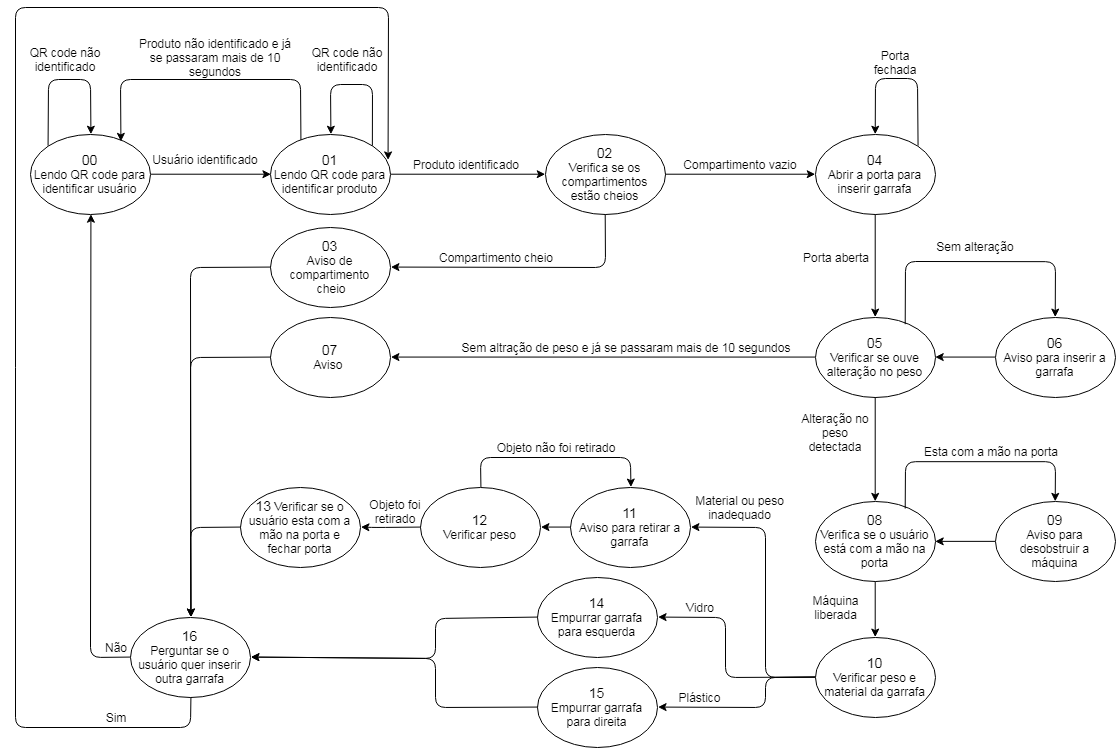
\includegraphics[scale=0.4]{figuras/eletronica/1-Maquina-de-estados.png}
	\caption{Máquina de estados de direcionamento das garrafas.}
\end{figure}

Primeiramente, no subsistema de separação de garrafas, existirá a etapa de reconhecimento do usuário através do QR code, onde o usuário fará o cadastro em um aplicativo (o desenvolvimento do aplicativo foi feito pela equipe de Engenheiros de Software), esse aplicativo por sua vez irá gerar um QR code que será lido pela máquina, então a máquina identifica o usuário. 

Ainda através de leitura de QR Code será feita a identificação do tipo de garrafa que será inserida na máquina, cada garrafa possui um QR code, o usuário vai ler esse QR code na máquina para que a mesma seja liberada para inserir a garrafa. O QR code em questão fornecerá alguns dos parâmetros relevantes para a preparação de reciclagem, tais como tipo de material da garrafa, peso médio, e para qual tratamento de preparação para reciclagem o material deve ser encaminhado. O sistema será gerido, de forma geral, através de um microcomputador Raspberry Pi 3.
 
O sistema irá verificar se o compartimento de armazenamento daquela garrafa está cheio e posteriormente acionar o controle de abertura e fechamento de um compartimento para que o usuário insira a garrafa a ser reciclada, aguardando até que o usuário insira a garrafa e que o compartimento seja desobstruído para evitar que a mão do usuário fique presa na máquina. Para verificar se a máquina está obstruída e se os compartimentos estão cheios foi utilizado sensores infravermelho reflexivos. 
 
Em seguida, ocorrerá a confirmação do tipo da garrafa e se a mesma está cheia de líquido ou vazia através de seu peso, além de uma possível nova confirmação do tipo de material da garrafa através de sensores capacitivos, com todos os dados contidos no código QR code lido anteriormente na garrafa, comparadas as informações contidas no banco de dados.  Estas confirmações serão realizadas através de uma célula de carga e possivelmente dois sensores capacitivos, que emitem uma resposta diferente dependendo do material da garrafa. Caso haja alguma não-conformidade na garrafa inserida, será emitido um aviso indicando a retirada da garrafa.
 
Após validada a garrafa inserida pelo usuário, a mesma será direcionada para o tratamento ideal, de acordo com o seu material de composição. Direcionamento este feito através de um fuso trapezoidal com movimentação baseada em um motor de passo. Caso a garrafa seja de plástico, a mesma será movida para o lado em que se possui o subsistema de trituração. Caso seja de vidro, a garrafa será movida para o lado que possui canaletas para armazenamento.  A capacidade de armazenamento será monitorada através de um sensor de presença (infravermelho).
 
Além do subsistema de separação de garrafas, o sistema eletrônico engloba também a parte de interação maquina-usuário. Inicialmente, através de leitura de QR code gerado pelo aplicativo e em seguida. Através de um display para exibir informações relevantes ao usuário, como por exemplo, nome do usuário e status de operação da máquina. Para isso, o sistema se utilizará também do microprocessador Raspberry Pi 3, e um display LCD 16x2.

Para alimentar todo o sistema até o momento está sendo utilizada uma fonte ATX de 250W. Para a alimentação final do sistema, o grupo referente a Engenharia de Energia ficou encarregado de construir uma fonte de alimentação. Fonte esta que deve ser capaz de suprir uma necessidade de potência de 50W , com saídas de 5V e 12V DC.
Medidas estas calculadas com base nas três principais fontes de consumo do subsistema em questão, ou seja, do microcomputador Raspberry Pi, microcontrolador ESP8266 e Motor de Passo. Abaixo, os consumos individuais acrescidos de um fator de segurança (Fs) de 1,35 visando possíveis alterações futuras do projeto, para o cálculo da potência total ativa.

\begin{equation}
    Potência\left ( W \right ) = Tensão\left ( V \right ) \ast Corrente\left ( A \right )
\end{equation}

\begin{equation}
    P_{Raspberry}\left ( W \right ) = T_{Raspberry}\left ( V \right ) \ast Corrente_{Raspberry}\left ( A \right )
\end{equation}

\begin{equation}
    P_{Raspberry}\left ( W \right ) = 5 \ast 2,5 = 12,5 \left ( W \right )
\end{equation}

\begin{equation}
    P_{ESP8266}\left ( W \right ) = T_{ESP8266}\left (V \right ) \ast Corrente_{ESP8266} \left ( A \right )
\end{equation}

\begin{equation}
    P_{ESP8266}\left ( W \right ) = 5 \ast 0,220 = 1,1 \left ( W \right )
\end{equation}

\begin{equation}
    P_{Motor de Passo}\left ( W \right ) = T_{Motor de Passo}\left (V \right ) \ast Corrente_{Motor de Passo} \left ( A \right )
\end{equation}

\begin{equation}
    P_{Motor de Passo}\left ( W \right ) = 12 \ast 2 = 24 \left ( W \right )
\end{equation}

\begin{equation}
    P_{Total}\left ( W \right ) = P_{Motor de Passo}\left (W \right ) + P_{Raspberry} \left ( W \right ) + P_{ESP8266} \left (W \right )
\end{equation}

\begin{equation}
    P_{Total}\left ( W \right ) = 12,5 * 1,1 * 24 = 37,6 \left ( W \right )
\end{equation}

\begin{equation}
    P_{FS}\left ( W \right ) = P_{Total}\left ( W \right ) * Fator de segurança
\end{equation}

\begin{equation}
    P_{FS}\left ( W \right ) = 36,7 * 1,35 \cong  50\left ( W \right )
\end{equation}

Sendo assim, um sistema de alimentação DC de 50 W com saídas de 5 e 12 V deverá ser utilizado, onde será suficiente para suprir todos os sistemas eletrônicos.

A arquitetura do sistema de direcionamento de garrafas pode ser observada na imagem a seguir.

\begin{figure}[!ht]
	\centering
		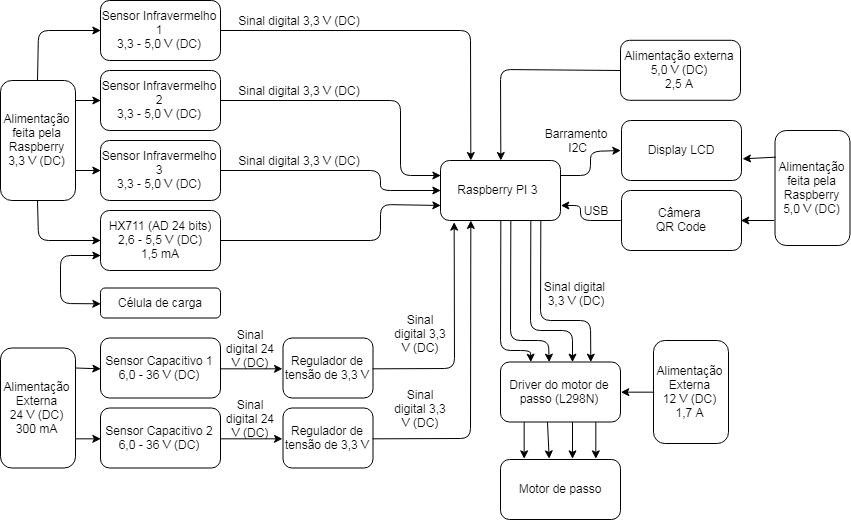
\includegraphics[scale=0.5]{figuras/eletronica/2-Arquitetura-do-direcionamento.png}
	\caption{Arquitetura do direcionamento de garrafas.}
\end{figure}

\subsection{Microprocessaodor}

O microprocessador utilizado foi a Raspberry PI 3, B, que possui um processador Quad Core de 1.2 GHz da Broadcom modelo BCM2837 de 64 bit, 1 GB de memória RAM, 4 portas USB, 1 saída HDMI, wireless LAN e Bluetooth, conector para display touchscreen e 40 pinos, dentre esses pinos temos entradas e saída digitais, interface I2C, interface SPI, interface UART e interface ID EEPROM, esses pinos podem ser programados de acordo com a necessidade de projeto. \cite{raspberryPi}

A sua escolha para o projeto se deu pelos seguintes motivos:

\begin{itemize}
    \item Versatilidade de programação, sendo possível programar em diferentes linguagens;
    \item Possuir uma quantidade suficiente de IOs (29 IOs) que podem ser configuradas tanto como entradas ou saídas digitais;
    \item Possibilidade da utilização de câmeras e displays (através de serial flat, usb, I2C ou SPI);
    \item Possuir Wi-Fi embutido, facilitando a comunicação via internet com o banco de dados;
    \item Fácil comunicação com diferentes microcontroladores e microprocessadores, garantindo assim uma possibilidade de  expansão, seja de processamento ou de acionadores através de mais IOs;
\end{itemize}

Assim, a Raspberry Pi 3 será o centro da arquitetura de automação e controle do subsistema de eletrônica, conforme indicado pela figura {\color{red} Arquitetura do direcionamento de garrafas} acima.

\begin{figure}[!ht]
	\centering
		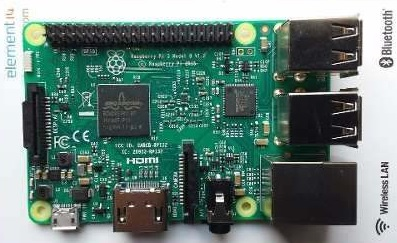
\includegraphics[scale=0.5]{figuras/eletronica/3-Raspberry-PI.jpg}
	\caption{Raspberry PI 3 modelo B.}
\end{figure}

\subsection{Display LCD}
Está sendo utilizado um display LCD 16x2 para exibir mensagens para o usuário, o mesmo foi escolhido pelo fato de um integrante do grupo já possuir um, ele se comunica com o microprocessador através do barramento I2C. Caso houvesse uma melhor condição econômica poderia ser escolhido um display melhor, como por exemplo um display em LCD de 9”, para que houvesse uma melhor interação entre a máquina e usuário. Mas como esta máquina é um protótipo, onde o importante é demonstrar o conceito de funcionamento do mesmo, o grupo optou por economizar recursos financeiros neste quesito.

\begin{figure}[!ht]
	\centering
		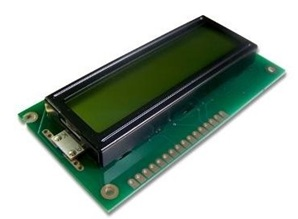
\includegraphics[scale=0.5]{figuras/eletronica/4-Display-LCD.jpg}
	\caption{Display LCD 16x2 utilizado no projeto.}
\end{figure}

\subsection{Motor de passo e driver}
O motor de passo escolhido foi o NEMA 17 com 3 Kgf/cm de torque, o mesmo foi escolhido devido ao fato de um integrante do grupo já possuir um, gerando economia financeira em relação ao orçamento do protótipo.

O motor de passo, é controlado pelo ativamento das bobinas, ou seja, tais motores não possuem escovas ou comutadores, apenas as bobinas que são polarizadas no sentido e no tempo certo para que haja um passo. O número de passos que é necessário para uma revolução é determinado pelo número de pólos que, dependendo, pode ser um imã ou um eletroímã em seu eixo, com eletroímãs em suas paredes. A velocidade de rotação e sentido são determinados pela forma como as bobinas são acionadas \cite{kalatec}.

\begin{figure}[!ht]
	\centering
		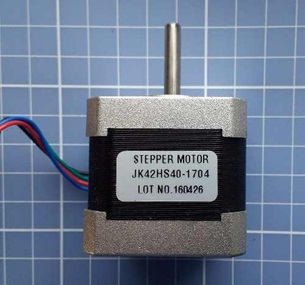
\includegraphics[scale=0.5]{figuras/eletronica/5-Motor-de-passo.jpg}
	\caption{Motor de passo NEMA 17 com 3 Kgfcm de torque, utilizado no projeto.}
\end{figure}

Para alimentar o motor de passo foi utilizada uma ponte H dupla, para isso foi utilizado o circuito integrado L298N, sua escolha foi devido ao preço e disponibilidade, já que o mesmo é encontrado facilmente nas lojas locais. Como o driver de corrente L298N é apenas uma ponte H dupla, toda a lógica de funcionamento do motor de passo foi feita na Raspberry Pi, assim como seu controle de velocidade, sentido de rotação e número de passos. 

Uma ponte H é formada basicamente por quatro transistores que permitem levar duas saídas para nível lógico alto ou baixo, com uma ponte H dupla como a que foi utilizada é possível controlar quatro saídas, sendo que no caso do L298N cada saída pode fornecer uma tensão de até 46 V e corrente de até 2 A suportando picos de corrente de até 3 A, como nosso motor de passo está sendo alimentado com 12 V e possui corrente nominal de 1,7 A, a ponte H dupla escolhida se enquadra nas especificações. 

\begin{figure}[!ht]
	\centering
		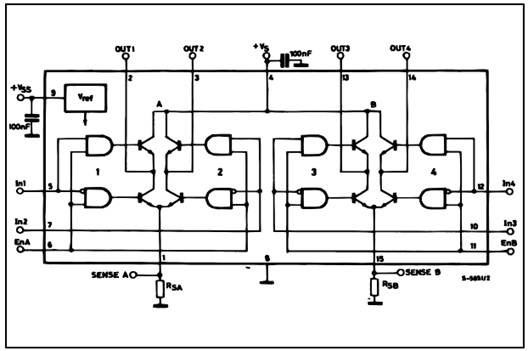
\includegraphics[scale=0.9]{figuras/eletronica/6-Diagrama-de-blocos-ponte-H.jpg}
	\caption{Diagrama de blocos da ponte H dupla (L298N) utilizada no projeto.}
\end{figure}

\begin{figure}[!ht]
	\centering
		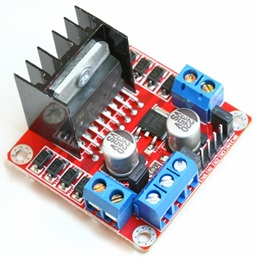
\includegraphics[scale=0.5]{figuras/eletronica/7-Ponte-H-dupla.jpg}
	\caption{Ponte H dupla L298N, utilizada no projeto.}
\end{figure}

\subsection{Sensor capacitivo}
São sensores capazes de detectar a aproximação de objetos sem a necessidade de contato físico, com princípio de funcionamento baseado na variação da capacitância. O sensor capacitivo é basicamente um capacitor de placas paralelas, onde o dielétrico é o material que se encontra na face do sensor, dessa forma, com a alteração do material dielétrico existe alteração na capacitância.\cite{tecnicasSensoriamento}

\begin{figure}[!ht]
	\centering
		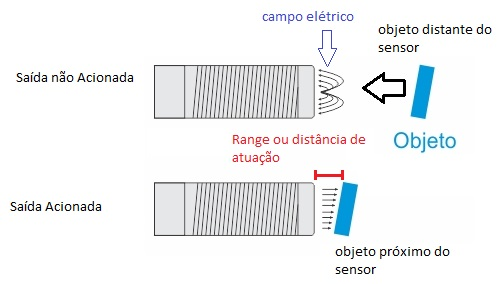
\includegraphics[scale=0.7]{figuras/eletronica/8-Funcionamento-sensor-capacitivo.jpg}
	\caption{Funcionamento do sensor capacitivo.}
\end{figure}

Funcionamento do sensor capacitivo. Fonte: \cite{sensorCapacitivoImagem}.

Composto por um capacitor de placas paralelas, o sensor capacitivo se baseia no princípio de mudança de frequência de oscilação de um circuito ressonante com a alteração do valor da capacitância, que por sua vez é causada pela mudança de dielétrico. A alteração de frequência é enviada a um circuito detector que transforma a variação de frequência em nível de tensão, um circuito trigger recebe esse sinal de tensão e o transforma em uma onda quadrada, que por sua vez é utilizada para excitar um circuito de potência, gerando um sinal digital de saída. \cite{sensorCapacitivo}

\begin{figure}[!ht]
	\centering
		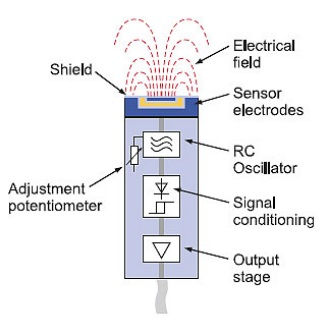
\includegraphics[scale=0.7]{figuras/eletronica/9-Partes-internas-sensor-capacitivo.jpg}
	\caption{Partes internas do sensor capacitivo.}
\end{figure}

Esse conjunto eletrônico que forma o sensor capacitivo é montado utilizando técnicas avançadas, sendo o conjunto alojado em invólucros metálicos com resina de alta densidade, formando um bloco sólido à prova d’água e vibrações. \cite{sensorCapacitivo}

O valor da capacitância de um capacitor de placas paralelas pode ser calculada através da equação a seguir, onde A é a área das placas, d é a distância entre as placas e epsilon é o valor da constante dielétrica. Como no caso do sensor capacitivo tanto A quanto d são constantes, a variação da capacitância será relacionada apenas com a variação do dielétrico.

\begin{equation}
    C = \varepsilon \frac{A}{d}
\end{equation}

O controle de qual dielétrico irá excitar a saída digital do sensor capacitivo é feito através de um potenciômetro, como já foi explicado anteriormente, dessa forma foi necessário utilizar dois sensores capacitivos no projeto, um para cada dielétrico, no caso plástico e vidro.

O sensor capacitivo escolhido foi o Ljc18a3-b-z/by Npn, o mesmo foi escolhido devido ao seu preço e disponibilidade, já que o mesmo foi encontrado em uma loja local. Este sensor é utilizado para detectar o material da garrafa que for inserida na máquina. O sensor funciona numa faixa de tensão de 6 até 36 V e possui uma saída digital que indica a presença de determinado material.

\begin{figure}[!ht]
	\centering
		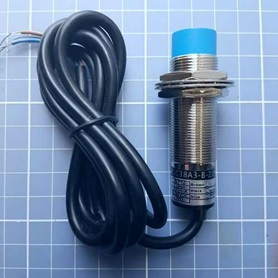
\includegraphics[scale=0.5]{figuras/eletronica/10-Sensor-capacitivo.jpg}
	\caption{Sensor capacitivo Ljc18a3-b-zby Npn.}
\end{figure}

\subsection{Célula de Carga}
A célula de carga escolhida foi do tipo SPL (single point) da marca IWM (International Weighing Manufacture) com capacidade máxima de 10 Kg, a mesma foi escolhida devido ao fato de um integrante do grupo já possuir uma. A sensibilidade desta célula de carga depende da tensão de excitação da célula, que é limitada entre a tensão recomendada (entre 6V e 10V) e a tensão máxima (15V), com a sensibilidade de 2mV/V. \cite{celulaCarga}.

\begin{figure}[!ht]
	\centering
		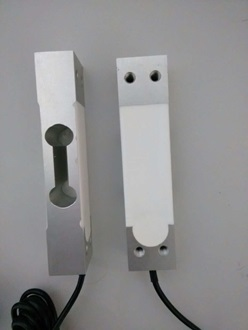
\includegraphics[scale=0.6]{figuras/eletronica/11-Celula-de-carga.jpg}
	\caption{Célula de carga utilizada no projeto.}
\end{figure}

\begin{figure}[!ht]
	\centering
		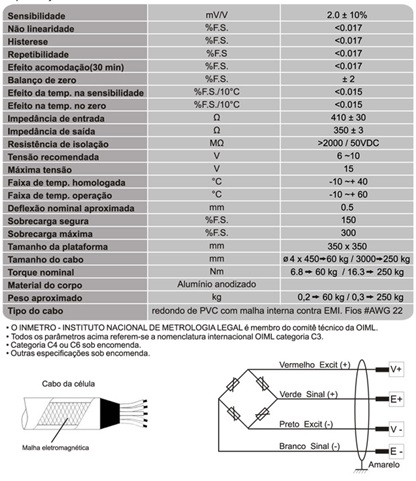
\includegraphics[scale=0.9]{figuras/eletronica/12-Informacoes-celula-carga.jpg}
	\caption{Informações da célula de carga.}
\end{figure}

Essa célula de carga possui dois extensômetros posicionados nas duas faces, superior e inferior. Para seu correto funcionamento um lado é fixado na estrutura e o outro lado é onde o esforço será aplicado, existe uma seta gravada na célula de carga indicando o sentido do esforço. 

O Extensômetro é um transdutor de deformação em resistência elétrica. Funciona a partir de trilhas de um fio em formato de grade, de maneira que ao se aplicar uma deformação, no sentido perpendicular a grade, o fio é esticado, diminuindo a área de seção transversal do mesmo aumentando assim a resistência, isso é possível observar na equação 2.38, que descreve a resistência em um fio, onde L é a largura do fio, A a área de seção transversal e rho a condutividade do material. \cite{extensometria}

\begin{equation}
    R = \rho \frac{L}{A}
\end{equation}

As deformações no fio são relacionadas pelo coeficiente de Poisson, a equação 2 mostra essa relação, tal que o coeficiente de Poisson é igual a deformação lateral dividida pela deformação coaxial do fio. \cite{extensometria}

\begin{equation}
    v = \frac{\varepsilon L}{\varepsilon a} (2)
\end{equation}

\begin{figure}[!ht]
	\centering
		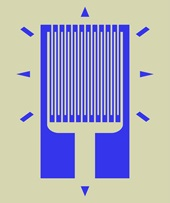
\includegraphics[scale=0.5]{figuras/eletronica/13-Extensometro.jpg}
	\caption{Extensômetro.}
\end{figure}

Para medir a variação de resistência é necessário outro transdutor de resistência para algum parâmetro como corrente ou tensão. A ponte de Wheatstone cujo esquemático é apresentado na figura a seguir, consegue relacionar o valor da resistência desconhecida a um valor de tensão, com as outras resistências tendo um valor fixo e preciso. A equação que relaciona as resistências a tensão entre os nós B e C é apresentada a seguir. É possível observar que se apenas uma das resistências for desconhecida o sistema tem apenas ela como variável. \cite{ponteWheatstone}

\begin{equation}
    VM = V * \frac{(R2R3 - R1R4)}{[(R1+R3)*(R2+R4)]} (3)
\end{equation}

\begin{figure}[!ht]
	\centering
		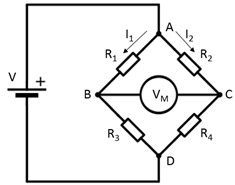
\includegraphics[scale=0.8]{figuras/eletronica/14-Circuito-da-Ponte-Wheatstone.jpg}
	\caption{Circuito da Ponte de Wheatstone.}
\end{figure}

Para tratar o sinal analógico proveniente da célula de carga está sendo utilizado o módulo HX711, esse módulo foi projetado para funcionar com pontes de winston, e já possui um conversor AD (analógico digital) de 24 bits, funciona com tensão de alimentação entre 2,6 e 5,5 V, a comunicação com o microprocessador é feita através de uma interface serial. \cite (interfacePonte). O módulo HX711 foi escolhido devido a seu preço, disponibilidade e funcionalidade, já que o mesmo foi projetado para funcionar com células de carga e já possui um conversor AD, sendo que a Raspberry PI não possui conversor AD.

\begin{figure}[!ht]
	\centering
		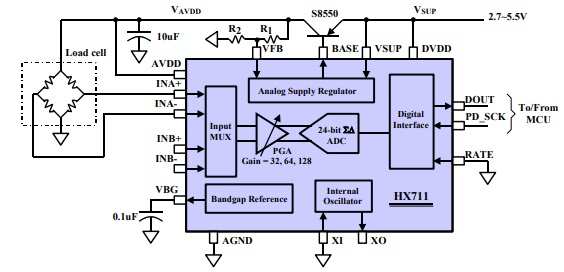
\includegraphics[scale=1.0]{figuras/eletronica/15-Diagrama-de-blocos-HX711.jpg}
	\caption{Diagrama de blocos da aplicação do HX711 com célula de carga.}
\end{figure}

\begin{figure}[!ht]
	\centering
		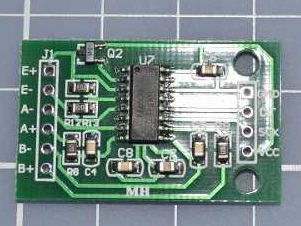
\includegraphics[scale=0.6]{figuras/eletronica/16-Modulo-HX711.jpg}
	\caption{Módulo HX711.}
\end{figure}

\subsection{Sensor infravermelho}
Este tipo de sensor possui um princípio de funcionamento muito simples, onde um LED emissor de luz infravermelha emite um feixe de luz que ao encontrar algum obstáculo é refletido, a luz refletida é detectada através de um fototransistor, quanto mais próximo ao obstáculo estiver o conjunto emissor/receptor maior será a intensidade do sinal recebido. \cite{sensoresOpticos}

\begin{figure}[!ht]
	\centering
		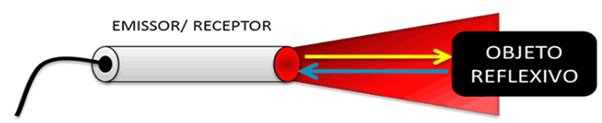
\includegraphics[scale=0.7]{figuras/eletronica/17-Principio-de-funcionamento-do-sensor-infravermelho-reflexivo.jpg}
	\caption{Princípio de funcionamento do sensor infravermelho reflexivo.}
\end{figure}

Para detectar se os compartimentos estão cheios, se o usuário está com a mão dentro da máquina ou se a garrafa foi mal inserida foi utilizado o sensor de obstáculo infravermelho por reflexão, o mesmo foi escolhido devido a sua funcionalidade, já que a distância de detecção do mesmo pode ser facilmente ajustada através de um potenciômetro, fornecendo uma saída digital que indica a presença de um objeto, apresentando uma solução simples para os problemas a serem solucionados, podendo ser encontrado facilmente em lojas locais a preços acessíveis. O sensor pode funcionar com tensão de alimentação entre 3,3 e 5 V e pode detectar obstáculos a distâncias de 2 até 30 cm, sendo que essa distância pode ser ajustada. \cite{sensorReflexivo}

\begin{figure}[!ht]
	\centering
		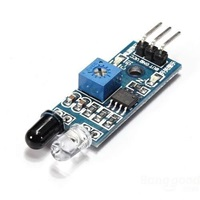
\includegraphics[scale=0.7]{figuras/eletronica/18-Sensor-de-obstaculo-infravermelho.jpg}
	\caption{Sensor de obstáculo infravermelho por reflexão utilizado no projeto.}
\end{figure}

\section{Acionamento do triturador}
O triturador não precisa ser acionado toda vez que uma garrafa plástica for inserida, como existe um funil, várias garrafas podem se acumular e quando chegar a um determinado nível, o triturador é acionado e tritura todas as garrafas presentes no funil. Dessa forma, foi desenvolvido um sistema de acionamento do triturador totalmente independente do sistema de direcionamento de garrafas, não existindo comunicação entre os sistemas.

Foi colocado um sensor infravermelho que funciona através de reflexão no topo do funil e um sensor infravermelho na parte de baixo do funil, assim é possível saber quando o funil está cheio para acionar o triturador, e quando todas as garrafas já foram trituradas resultado no desligamento do triturador e acionamento do freio do motor do triturador.

Para acionar o motor e o freio do motor, foram utilizados dois relés com tensão nominal de 250 V (AC) e 10 A, a especificação da corrente e tensão desses relés foi feita pelos membros do grupo pertencentes a Engenharia de Energia. Sendo assim foi comprado um módulo relé que já contém os dois relés necessários para realizar o controle do motor, sendo que este módulo já está equipado com um optoacoplador para evitar que o microcontrolador possa sofrer danos.

Para realizar o controle do acionamento e frenagem do motor foi utilizado o microcontrolador ESP8266, o mesmo foi escolhido pelo fato de um membro do grupo já possuir a placa. O ESP8266 é possui Wi-Fi embutido, Tem onze portas GPIO, barramentos I2C, SPI, UART, conversor AD, saída PWM, processador L106 32-bit que funciona a 80 MHz, 32 KBytes de RAM para instruções, 96 KBytes de RAM para dados, 64 KBytes de ROM para boot, possui uma memória Flash SPI Winbond W25Q40BVNIG de 512 KBytes, é fabricado pela Espressif. \cite{microESP}

Na imagem a seguir é possível visualizar a topologia do sistema de controle do motor, onde o microcontrolador ESP8266 recebe os sinais dos dois sensores infravermelho e aciona os relés para ligar o triturador e frear o motor.

\begin{figure}[!ht]
	\centering
		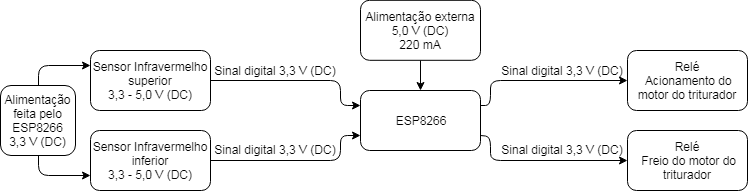
\includegraphics[scale=0.6]{figuras/eletronica/19-Arquitetura-do-controle-e-acionamento-do-motor.png}
	\caption{Arquitetura do controle e acionamento do motor.}
\end{figure}

Para realizar o controle do acionamento e frenagem do motor foi feita uma modelagem através de máquina de estados, que facilita o entendimento do funcionamento sistema. Como é possível visualizar na imagem a seguir.

\begin{figure}[!ht]
	\centering
		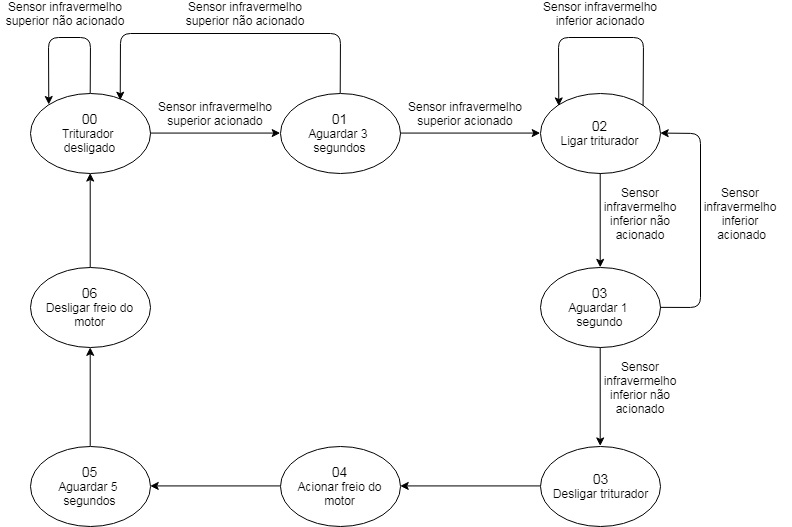
\includegraphics[scale=0.5]{figuras/eletronica/20-Maquina-de-estados-do-controle-de-acionamento-e-frenagem-do-triturador.png}
	\caption{Máquina de estados do controle de acionamento e frenagem do triturador.}
\end{figure}

Como é possível visualizar na imagem, inicialmente o motor está desligado e o sistema está lendo o sensor infravermelho superior, quando algo é detectado por este sensor é aguardado 3 segundos e o mesmo sensor é verificado novamente, isso é necessário pois quando a garrafa cai dentro do funil ela passa pelo sensor e aciona o mesmo, sendo assim, com essa segunda verificação é possível saber que existe uma garrafa naquele ponto do funil e não que a garrafa apenas passou por ali. 

Posteriormente o triturador é ligado, com o motor ligado o sensor infravermelho localizado na parte inferior do funil é verificado constantemente, quando o mesmo não detecta mais a presença de garrafas é aguardado um segundo e realizada uma segunda verificação para evitar que a garrafa “pule” enquanto está sendo triturada e ocasione o desligamento do triturador, depois dessa segunda verificação o triturador pode ser desligado.

Após o desligamento do motor é acionado o freio do motor por corrente contínua, são aguardados 5 segundos (esse tempo ainda será definido através de testes práticos, a equipe responsável por definir o tempo que o freio ficará acionado é a equipe de Engenheiros de Energia), após esse tempo o freio é desligado e a máquina retorna a seu estado inicial.

\begin{figure}[!ht]
	\centering
		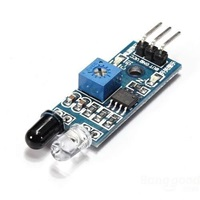
\includegraphics[scale=0.8]{figuras/eletronica/21-Sensor-de-obstaculo-infravermelho-reflexao-p-deteccao-garrafas-no-funil.jpg}
	\caption{Sensor de obstáculo infravermelho por reflexão utilizado para detecção de garrafas no funil.}
\end{figure}

\begin{figure}[!ht]
	\centering
		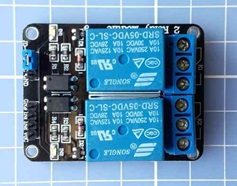
\includegraphics[scale=0.7]{figuras/eletronica/22-Modulo-rele-de-2-canais.jpg}
	\caption{Módulo relé de 2 canais (250 V AC 10 A) utilizado para acionamento do triturador e freio do moto.}
\end{figure}

\begin{figure}[!ht]
	\centering
		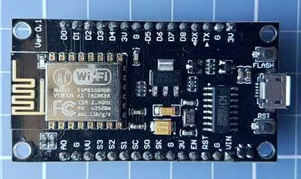
\includegraphics[scale=0.7]{figuras/eletronica/23-Microcontrolador-ESP8266.jpg}
	\caption{Princípio de funcionamento do sensor infravermelho reflexivo.}
\end{figure}

\section{Integração}
\begin{figure}[!ht]
	\centering
		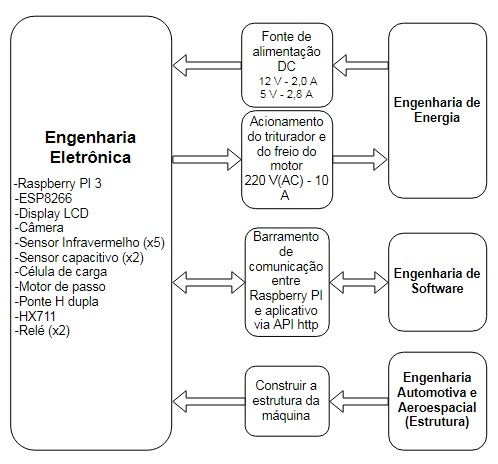
\includegraphics[scale=0.8]{figuras/eletronica/24-Diagrama-de-integracao.jpg}
	\caption{Diagrama de integração entre a Engenharia Eletrônica e as demais áreas.}
\end{figure}

\subsection{Engenharia de Energia}
É necessário que esta área forneça alimentação DC para o correto funcionamento do sistema eletrônico, como explicado anteriormente, será necessário uma fonte DC de 45 W com saídas de 5 V/2,8 A e 12 V/2 A. Além da especificação dos relés de acionamento do motor e freio, cujas especificações informadas foram para ambos 250 V (AC) 10 A, e do tempo em que o freio deverá permanecer acionado.

Será fornecido para Engenharia de energia a saída para acionamento do motor e do freio através de dois relés já especificados, todo o controle de acionamento e frenagem ficou por conta da Engenharia Eletrônica. 

\subsection{Engenharia de Software}
A integração entre o subsistema de Eletrônica e o de Software é de imensa importância, tendo em vista que toda associação máquina e usuário é feita por essa união. Após o Subsistema de Eletrônica realizar a leitura e processamento do QRcode do usuário e o da garrafa, essa informação é enviada para API do Subsistema de Software, via http post, utilizando a Raspberry PI 3 como responsável por encaminhar a mensagem. A resposta da requisição http post retorna os dados necessário para que o Subsistema de Eletrônica possa fazer a comparação das variáveis recebidas pela requisição http post e por meio das medições realizadas pelos sensores. 

Quando o Subsistema de Eletrônica encaminhar a string referente ao processamento do QRcode da garrafa, o Subsistema de Software deve retornar as informações referentes ao material da garrafa, peso e label. Já quando Subsistema de Eletrônica encaminha a string referente ao usuário, será recebido o retorno via http post dos dados cadastrais do mesmo. 

\subsection{Estrutura}
Está área do conhecimento deverá fornecer para engenharia eletrônica a estrutura de seleção (já entregue) e a estrutura geral da máquina, com locais adequados para que sejam acomodados os sensores, atuadores, microcontroladores e fonte de alimentação.

A Engenharia Eletrônica forneceu as dimensões exatas de todos os seus componentes, onde eles devem ficar alocados, além de informar suas restrições e requisitos de funcionamento.

\section{Testes}
Até o momento, diversos testes de adequação e funcionamento foram realizados por parte do subgrupo de engenharia eletrônica, relacionados à componentes como motor de passo, sensores capacitivos e infravermelho, além de processamento de imagens na Raspberry Pi 3 e uso de célula de carga.

Sobre o motor de passo, foram realizados testes individuais, com o motor livre de qualquer tipo de fixação ou estrutura para verificar movimentação básica. Seguido de testes com o motor, driver e Raspberry Pi já posicionados na estrutura da máquina, onde foi possível se verificar velocidade e quantidade de passos ideais para que o modo operacional inicialmente idealizado seja de possível realização. A partir destes testes,foi possível também fazer ajustes na estrutura, como por exemplo limitação de tamanho de tampa frontal móvel e de ajuste no fuso de movimentação.

Quanto ao processamento de imagens na Raspberry Pi, foram realizadas as devidas instalações de drivers e construção de código em Python para possibilitar a leitura de vídeo em tempo real através de uma webcam USB, para que em seguida testes de leitura de QR code sobre tela de smartphone fossem executados, a fim de verificar viabilidade e ajustes como relação entre qualidade e framerate de buffer de vídeo e fatores como brilho de tela por parte do smartphone. Além disso, foram realizados testes com impressão de QR Codes para fixação em garrafas de plástico e vidro, em diversos tamanhos e qualidades de impressão, a fim de verificar a condição ideal para a leitura dos mesmos. Ao fim destes testes, foi possível verificar que é possível diminuir de forma considerável o framerate de leitura via webcam, que o brilho de tela em smartphones não necessitam de mais de cerca de  20\% a 30\% de brilho máximo para uma leitura ideal, e se ter noção do tamanho e qualidade de impressão mínimos para uso do QR Code em garrafas.

Já em relação aos sensores capacitivos, foram realizados testes em bancada com fonte de tensão variável, a fim de verificar qual era a relação entre acréscimo de tensão e sensibilidade adquirida pelo sensor, tendo em vista que o mesmo opera em um raio de 6 à 36 Volts. Além disso, estes sensores foram testados com diferentes distâncias e tipos de garrafas de vidro e plástico, que são os materiais de interesse do protótipo em questão, e verificou-se o comportamento destes sensores na presença de resquícios de líquido. A partir dos resultados destes testes, concluiu-se que a tensão ideal para seu funcionamento é de 12 Volts, e que as garrafas devem estar bem próximas do sensores para uma leitura ideal, pois o alcance do mesmo é de 10 milímetros. Sendo assim, foi requisitado para o subgrupo de estruturas para se adicionar uma leve inclinação no compartimento onde as garrafas serão inseridas, visando sempre uma distância mínima entre sensores capacitivos e garrafas a serem analisadas pelos mesmos. 
Ainda sobre sensores capacitivos, verificou-se também que fatores como líquidos presentes nas garrafas podem dificultar a precisão em determinar que tipo de material se está inserindo no equipamento, devido à água alterar a resposta do sensor capacitivo, e pelo fato da qualidade do sensor utilizado no protótipo, que não possui um grande orçamento planejado. Mas, como um dos requisitos de funcionamento do triturador de garrafas plásticas é de não poder receber garrafas com líquidos, este problema é facilmente resolvido utilizando a célula de carga, realizando a comparação dos pesos da garrafa (QRcode e balança).

Sobre os sensores infravermelhos, testes de adequação foram também realizados, visando questões práticas como distância mínima para ponto de interesse de detecção e tipos de materiais suportados pelo sensor. Como resultado dos testes, constatou-se que os sensores funcionam em detecção de objetos a distâncias suficientes em termos do projeto em questão, e em sua única limitação quanto a tipos de materiais, o sensor mostrou não funcionar de maneira ideal quando frente à objetos de cor preta, mas que dentro das diretrizes de funcionamento do protótipo, esta não será uma limitação em seu uso.

Por fim, realizou-se testes com célula de carga com programação e calibrações baseadas em programação python na Raspberry Pi. Testes estes que nos entregaram variações de no máximo 5 gramas nos pesos testados, e que, sendo assim, o componente mostra que irá atender às necessidades impostas pelos requisitos do protótipo.


